\chapter{Product Assurance}

\section{Overview}

The prime objective of product assurance is to ensure that space products accomplish their defined mission objectives in a safe, available and reliable way. In support of project risk management, product assurance assures an adequate identification, appraisal, prevention and control of technical risks within project constraints.

\section{Product Assurance Disciplines}

In order to implement the product assurance process, a number of disciplines are involved. They are described in the following sections.

\subsection{Product Assurance Management}

\begin{tabular}{l}
\textit{ECSS-Q-ST-10 "Product assurance management" \cite{ECSS-Q-ST-10}}
\end{tabular}

Product assurance management is a multidisciplinary activity to ensure that a product assurance program is implemented and managed throughout all project phases and coordinated with all actors. It addresses the \textbf{product assurance plan} (Section \ref{sec:Product Assurance Plan}) defining all product assurance activities consistent with the project objectives, requirements, criticalities and constraints. 

In particular it includes the allocation and availability of adequate resources, personnel and facilities to carry out the necessary tasks and to follow up progress monitoring, reporting and visibility of all product assurance matters, in particular those related to alerts, critical-items, nonconformances, changes, deviations, waivers, actions or recommendations resulting from reviews, inspection and audits, qualification, verification and acceptance.

The product assurance (PA) manager shall ensure that a \textbf{qualification status list} (Section \ref{sec:Qualification Status List}) is maintained throughout the project lifetime.

\subsubsection{Critical-Item Control}
\label{sec:Critical-Item Control}

\begin{tabular}{l}
\textit{ECSS-Q-ST-10-04 "Critical-item control" \cite{ECSS-Q-ST-10-04}}
\end{tabular}

Critical items (CI) are potential threats to the performance, quality, dependability and safety of a system that are controlled by a specific action plan in order to mitigate emanating risks and to prevent undesirable consequences. Such items shall be formally identified and controlled in a \textbf{critical-item list} (Section \ref{sec:Critical-Item List}). 

Various product assurance analyses provide considerable inputs for identification of critical items (e.g. RAMS: FMECA results, hazard analysis results; PMP: non-qualified parts, materials and processes; EEE: non-qualified parts or new technology; lessons learned from previous programs). Annex C of ECSS-Q-ST-10-04 provides a guide for identifying critical items.

The control process for critical items is similar to the risk management process and bears interface to it, namely:

\begin{itemize}
\item critical-item inputs to the risk identification activity, 
\item risk classifications used to prioritize critical items, 
\item references between risk reduction and critical item control measures, 
\item status of critical-item control implementation. 
\end{itemize}

In addition to the critical-item list, \textbf{critical-item control forms} (Section \ref{sec:Critical-Item Control Form}) shall be created and maintained by the PA manager.

\subsubsection{Nonconformance Control}
\label{sec:Nonconformance Control}

\begin{tabular}{l}
\textit{ECSS-Q-ST-10-09 "Nonconformance control system" \cite{ECSS-Q-ST-10-09}}
\end{tabular}

Whenever in the project lifetime a nonconformance is detected, the product assurance representative shall analyse and document it in a \textbf{nonconformance report} (Section \ref{sec:Nonconformance Report}). This report is then to be submitted to the internal nonconformance review board (NRB) for assessment, which classifies it as either minor or major, and maintains a list of all identified nonconformance items and their status (Section \ref{sec:NCR Status List}).

Major nonconformances are those that have an impact on safety, reliability, maintainability, lifetime, interchangeability, or on operational, functional, or contractual requirements.

Minor and major nonconformances are disposed in either of the following ways: return to supplier (for procured items), use "as-is", rework, scrap, or repair. The difference between handling of minor and major nonconformances is that minor ones are decided and acted upon within the project team, whereas major ones have to be addressed together with the customer.
 
Although ECSS-Q-ST-10-09 also covers operational nonconformances during mission operations phase, these are better to be handled with dedicated anomaly reports as discussed in Section \ref{sec:Operations Reporting}.

\subsection{Quality Assurance}

\begin{tabular}{l}
\textit{ECSS-Q-ST-20 "Quality assurance" \cite{ECSS-Q-ST-20}}
\end{tabular}

Quality assurance (QA) is the main pillar of product assurance. Quality assurance management focuses on ensuring the quality throughout the design, verification, procurement, manufacturing, assembly, integration, testing, acceptance, and delivery of the product. The \textbf{quality assurance plan} (Section \ref{sec:Quality Assurance Plan}) provides details on all these aspects. 

In addition, a documented training/certification plan shall be established for personnel, whose performance determines or affects product quality, and records of such trainings shall be maintained.

The quality assurance comprises the following phase-independent activities:

\begin{itemize}
\item critical-items control (Section \ref{sec:Critical-Item Control})
\item nonconformance control (Section \ref{sec:Nonconformance Control})
\item alert management 
\item stamp control
\item traceability 
\item metrology and calibration 
\item handling, storage and preservation

\end{itemize}

An \textbf{alert management system} is used to inform the customer on issues that are detected and that do not fall under nonconformance category, with possibly impact on other projects. Typically this is for (generic) software applications or support equipment. An incident management system can be used for this.

\textbf{Stamp control} refers to methods of implementing a correct and legitimate authorizations system, to ensure, for example, that digital signatures are protected and trustful.

\textbf{Traceability} means that there is maintained a relationship between parts, materials, or products and their associated documentation. This is largely covered in Section \ref{sec:Configuration Management}.

Broadly speaking, \textbf{metrology and calibration} refers to proper control, calibration and maintenance of measurement and test equipment. 

For the \textbf{handling, storage and preservation} of items, proper means shall be established to prevent damages during all phases, from manufacturing to operations. ECSS-Q-ST-20-08 \cite{ECSS-Q-ST-20-08} addresses this for spacecraft hardware in detail.

\subsubsection{Design and Verification}

Quality assurance principles for design and verification phase comprise the definition of design rules and methods, the selection of tools, and to ensure that the design is producible and repeatable.

The use of \textbf{space qualified parts} in system design significantly adds to the quality of the system in terms of reliability. The ESCC (European Space Components Coordination) for example publishes a list of components and technologies which have been, respectively, qualified and capability approved by ESA \cite{spacecomponents.org}.

Another aspect of quality assurance covers the use of \textbf{off-the-shelf} (OTS) hardware items as addressed in ECSS-Q-ST-20-10 \cite{ECSS-Q-ST-20-10}, namely those that have not yet been qualified for space applications. OTS items are those that, even if not necessarily developed for space applications, can be procured from the market and utilized in a space system. For CubeSat missions this typically forms a large part of items that make up the spacecraft system. It is therefore not foreseen to make a strict distinction between such items, and rather focus on extensive testing and verification on all levels and various stages, as discussed in Section \ref{sec:Verification}.

\subsubsection{Procurement}

The procurement activity shall be controlled to ensure that all items and services
procured conform to technical and quality assurance requirements. The control of procurement activity includes selection of procurement sources, control of purchase documents, and inspection of incoming items.

\subsubsection{Manufacturing, Assembly and Integration}

All manufacturing processes shall be covered by documented process specifications or standards. In particular ECSS-Q-ST-70 \cite{ECSS-Q-ST-70} provides a number of process standards for manufacturing. In addition, workmanship standards shall be defined and applied throughout all phases. This also comprises requirements for cleanliness as detailed in ECSS-Q-ST-70-01 \cite{ECSS-Q-ST-70-01}.

Further, \textbf{logbooks} shall be maintained on system, subsystem, and equipment level (Section \ref{sec:Logbook}) that document all operations and tests performed on the item during the period to be covered by the logbook.

\subsubsection{Testing}

Quality assurance shall ensure that internal and external test facilities conform to specified requirements. Details on quality assurance for test centers are provided in ECSS-Q-ST-20-07 \cite{ECSS-Q-ST-20-07}.

QA shall also ensure that test documentation is done properly, comprising test procedures and test reports. QA personnel shall monitor test executions where needed and attend test reviews.

\subsubsection{Acceptance and Delivery}

Quality assurance shall ensure the preparation of an \textbf{end item data package} (Section \ref{sec:End Item Data Package}) for each deliverable and monitor the actual process of delivering to ensure no degradation of quality to the item.

\subsection{Dependability}

\begin{tabular}{l}
\textit{ECSS-Q-ST-30 "Dependability" \cite{ECSS-Q-ST-30}}
\end{tabular}

The dependability discipline addresses all aspects to ensure that the dependability performance (availability performance and its influencing factors reliability performance, maintainability performance and maintenance support performance) is met for the space product. That means that even in case of error the system shall continue to function, to certain extent. In particular it includes design rules (e.g. derating, end of life parameter drifts) and dependability analysis (e.g. worst case circuit performance, failure mode and effects, criticality).

\subsubsection{Dependability Engineering}

Dependability aspects shall be considered already in the process of requirements engineering, and shall include:

\begin{itemize}
\item design performance margins
\item derating factors
\item human factor influences
\item fault tolerance to hardware failures or software malfunctions
\item redundancies and system simplifications
\item detection, isolation, diagnosis, and recovery of the system from failures
\item monitoring of essential mission performance parameters
\end{itemize}

\textbf{Derating} means to design a system such that its components operate at a significantly reduced level of stress to increase reliability and to ensure useful life and design margins (see ECSS-Q-ST-30-11 \cite{ECSS-Q-ST-30-11}).

In support of achieving dependable design, the definition of \textbf{success criteria} on each level of the system shall be defined.

Further, the classification of severity levels shall be defined and assigned to each identified failure mode and failure effect. Typical severity levels are:

\begin{enumerate}
\item Catastrophic (everything more severe than loss of mission)
\item Critical (loss of spacecraft)
\item Major (major mission degradation)
\item Minor (minor mission degradation or other)
\end{enumerate}

\subsubsection{Dependability Analyses}

Dependability analyses shall be conducted on all levels of the space system. There exist a number of different categories of analyses.

\textbf{Reliability analyses} make up the dominant category of dependability analyses and deal with analysing uncertainties and risks of failure. Common reliability analyses are:

\begin{itemize}
\item \textbf{FMEA/FMECA}: Failure modes and effects analyses / failure modes, effects and criticality analyses identify potential failure modes and associate a severity or criticality level to it. See ECSS-Q-ST-30-02 \cite{ECSS-Q-ST-30-02} for details.
\item \textbf{HSIA}: Hardware-software interaction analysis, as part of FMEA/FMECA.
\item \textbf{Contingency analyses}: Identify system level failures and indicate how to recover the system.
\item \textbf{FTA}: Fault tree analysis ensures that the design conforms to the failure tolerance requirements for combination of failures. See ECSS-Q-ST-40-12 \cite{ECSS-Q-ST-40-12} for details.
\item \textbf{WCA}: Worst case analysis shall be performed on electrical equipment to demonstrate that it performs within specification under (externally and/or internally implied) worst case conditions. See ECSS-Q-HB-30-01 \cite{ECSS-Q-HB-30-01} for details.
\item \textbf{FDIR}: Failure detection, isolation and recovery analysis shall be performed at system level to ensure that autonomy and failure tolerance requirements are fulfilled. See ECSS-E-ST-70-11 \cite{ECSS-E-ST-70-11} for details.
\end{itemize}

In addition, \textbf{part stress analyses} (verify that derating rules have been implemented correctly) and \textbf{zonal analyses} (problems due to potential subsystem-to-subsystem interactions) may be carried out where needed.

The other two categories of analyses are \textbf{maintainability analyses} and \textbf{availability analyses}. These include mean time before failure (MTBF) and mean time to repair (MTTR) analyses. See ECSS-Q-ST-30-09 \cite{ECSS-Q-ST-30-09} for details on availability analyses.

\subsection{Safety}

\begin{tabular}{l}
\textit{ECSS-Q-ST-40 "Safety" \cite{ECSS-Q-ST-40}}
\end{tabular}

The safety discipline shall ensure that all safety risks associated with the design, development, production and operations of the space system are identified, assessed, minimized, controlled and finally accepted through the implementation of a safety assurance program. The objective is to ensure that the space system does not cause a hazard to, in order of priority:

\begin{enumerate}
\item Human life
\item Environment
\item Public and private property
\item Spacecraft and launcher
\item Ground support equipment and facilities
\end{enumerate}

The safety program is detailed in the \textbf{safety program plan} (Section \ref{sec:Safety Program Plan}). The safety manager is responsible for ensuring that \textbf{safety risks} are identified and properly controlled (via the risk management process, see Section \ref{sec:Risk Management}), and that \textbf{safety training} and \textbf{accident-incident reporting} is properly implemented.  

The most essential tools available to ensure safety are the hazard analysis and fault tree analysis.

\subsubsection{Hazard Analysis}

\begin{tabular}{l}
\textit{ECSS-Q-ST-40-02 "Hazard analysis" \cite{ECSS-Q-ST-40-02}}
\end{tabular}

A hazard is an existing or potential condition of an item that can result in a mishap. For example, the use of Lithium-Ion batteries on a CubeSat are a hazard as they are a potential threat to the safety of the system (an associated hazard scenario would be the explosion of the battery). Hazards therefore present safety risks, which in turn is a subcategory of risks. Due to their nature, they are to be identified, recorded, and controlled in a dedicated manner as outline in the following.

Similar to the risk management process, the hazard analysis process follows the following pattern:
Define analysis requirements
$\rightarrow$ Identify and classify
$\rightarrow$ Decide and act
$\rightarrow$ Close or track
$\rightarrow$ Identify and classify
$\rightarrow$ etc.

Hazards (e.g. explosiveness) are present in the system through hazard manifestation (e.g. lithium-ion battery technology implemented). They are activated through initiating causes (e.g. battery short circuit), then result in the event (e.g. high current flow, pressure build up), and finally lead to a consequence (e.g. loss of power supply, damage to system). Figure \ref{fig:Example of Hazards and Hazard Scenarios} shows an example. Different scenarios can originate from the same hazard, while different scenarios can also lead to the same safety consequences.

\begin{figure}[h]
\centering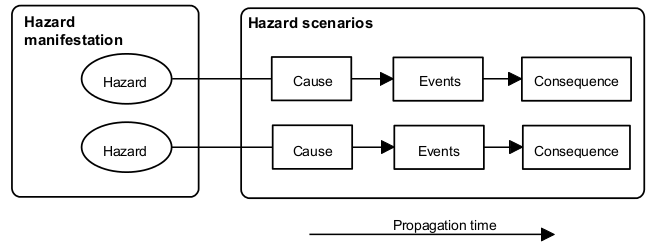
\includegraphics[scale=0.6]{fig/example_of_hazards_and_hazard_scenarios}
\caption{Example of Hazards and Hazard Scenarios (ECSS)}
\label{fig:Example of Hazards and Hazard Scenarios}
\end{figure}

Hazards are reduced by either eliminating them or, if not feasible, by minimizing and controlling them (see Figure \ref{fig:Removal or Change of Hazards, Elimination of Event, or Interruption of Event}). 

\begin{figure}[h]
\centering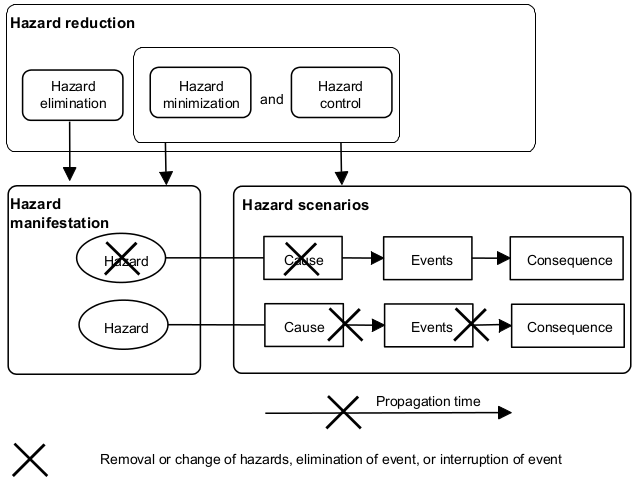
\includegraphics[scale=0.6]{fig/removal_or_change_of_hazards}
\caption{Removal or Change of Hazards, Elimination of Event, or Interruption of Event (ECSS)}
\label{fig:Removal or Change of Hazards, Elimination of Event, or Interruption of Event}
\end{figure}

\subsubsection{Fault Tree Analysis}

\begin{tabular}{l}
\textit{ECSS-Q-ST-40-12 "Fault tree analysis" \cite{ECSS-Q-ST-40-12}}
\end{tabular}

Fault tree analysis (FTA) is a top-down method that stipulates a fault and tries to identify causes to led to this fault. This is done downwards the system levels until the root causes are found. This is in contrast with failure mode and effects analysis (FMEA), which is an inductive, bottom-up analysis method aimed at analyzing the effects of single component or function failures on the next higher system. 

\begin{figure}[h]
\centering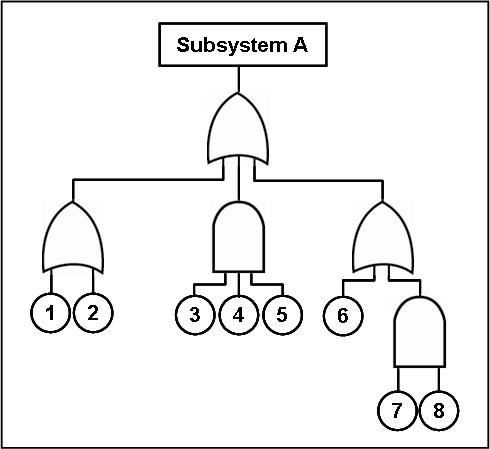
\includegraphics[scale=1.0]{fig/example_of_fault_tree_analysis}
\caption{Example of Fault Tree Analysis}
\label{fig:Example of Fault Tree Analysis}
\end{figure}

\subsubsection{Space Sustainability}

The system design and operation shall be such as to minimize \textbf{debris mitigation}, which pose a potential collision hazard to other objects in space. See ECSS-U-AS-10 \cite{ECSS-U-AS-10} for an adoption note of the ISO 24113 standard on space debris mitigation requirements. \textbf{Atmospheric re-entry} on the other hand poses a risk to people, environment, and property.

\subsection{EEE Components}

The electrical, electronic and electromechanical (EEE) components discipline defines some specific requirements for selection, control and procurement of EEE components for space projects to ensure that they satisfy the mission performance requirements during the full life cycle of the products.  

ECSS-Q-ST-60 \cite{ECSS-Q-ST-60} differentiates between three classes of components, from class 1 with highest assurance and lowest risk, to class 3 with lowest assurance and highest risk. The standard then defines the requirements for components of those three classes. ECSS-Q-ST-60-13 \cite{ECSS-Q-ST-60-13} extends this standard further, by tailoring and modifying its requirements with application to commercial off-the-shelf (COTS) components. 

For typical CubeSat missions even class 3 requirements are in most cases much too demanding. Nonetheless, it is good practice to check against the availability of space qualified components, such as published at the website of the European Space Components Information Exchange System (ESCIES) \cite{escies.org}. 

Further, a \textbf{declared component list} (DCL) (Section \ref{sec:Declared Component List}) shall be maintained that provides a status list of all the EEE components intended to be used or actually used in the system.

As mentioned, mainly COTS EEE components are employed in CubeSat missions. For designs that implement such components of which some or all are not space qualified (i.e. they do not carry heritage from flown space missions), the following aspects shall be taken into special account: 

\begin{itemize}
\item \textbf{Temperature range}: Commercial parts shall be selected in the highest available temperature range and shall have a minimum margin of $10\,^{\circ}\mathrm{C}$.
\item \textbf{Radiation}: Survival and successful operation of space systems in the space radiation environment cannot be ensured without careful consideration of the effects of radiation, namely the effects of total ionizing dose (TID), total non-ionizing dose (TNID) and single-event effects (SEE). ECSS-Q-ST-60-15 \cite{ECSS-Q-ST-60-15} provides details on radiation hardening assurance. ECSS-E-HB-10-12 \cite{ECSS-E-HB-10-12} provides details on calculation of radiation and its effects.
\end{itemize}

\subsection{Materials, Parts and Processes}

\begin{tabular}{l}
\textit{ECSS-Q-ST-70 "Materials, mechanical parts and processes" \cite{ECSS-Q-ST-70}}
\end{tabular}

The materials, mechanical parts and processes discipline defines requirements for selection, control and procurement of materials, mechanical parts and processes for space projects to ensure that they satisfy the mission performance requirements during the full life cycle of the products. 

The following lists are to be prepared and maintained for all the configuration items in the system:

\begin{itemize}
\item \textbf{Declared materials list (DML)}: A detailed record of all the materials used to produce the products of the space system. To obtain this list, one may need to access the composition of parts in terms of materials (Section \ref{sec:Declared Materials List}).
\item \textbf{Declared mechanical parts list (DMPL)}: A detailed record of all the mechanical parts used to produce the products of the system. The bill of material (BOM) of products can be used to derive this information (Section \ref{sec:Declared Mechanical Parts List}).
\item \textbf{Declared process list (DPL)}: A detailed record of all the processes used to produce the products of the space system (Section \ref{sec:Declared Process List}).
\end{itemize}

A helpful guideline for the selection of materials and definition of processes is provided in ECSS-Q-ST-70-71 \cite{ECSS-Q-ST-70-71}.

\subsubsection{Cleanliness}

\begin{tabular}{l}
\textit{ECSS-Q-ST-70-01 "Cleanliness and contamination control" \cite{ECSS-Q-ST-70-01}}
\end{tabular}

The purpose of cleanliness and contamination control is to avoid malfunctions and failures of hardware items due to particulate or molecular contamination. The classification of \textbf{particulate contamination levels} is done in ISO Class levels from 1 to 9, with ISO Class level 1 being the cleanest. The levels specify the maximum concentration of particles of different sizes per air volume.

The requirements on \textbf{cleanrooms} are provided in detail and govern the design aspects of the cleanroom, the air supply, the filters, the air monitoring, the temperature control, the pressure control, and the humidity control. It also specifies on how to verify the cleanroom cleanliness levels. The maintenance, cleaning, and access control to the cleanroom are specified as well. ECSS-Q-ST-70-50 \cite{ECSS-Q-ST-70-50} provides more detail on \textbf{monitoring of contamination} for space systems and cleanrooms.

Appendix D and E of ECSS-Q-ST-70-01 provide guidelines for \textbf{general cleanliness and contamination control} and on \textbf{cleanliness-oriented design}. Appendix I of ECSS-Q-ST-70-01 provides an matrix of compatibility of \textbf{cleaning solvents} and target materials. Appendix M of ECSS-Q-ST-70-01 provides an informative guide on \textbf{cleaning methods} for removal of particulate and molecular contamination.

\subsubsection{Material Testing}

Several ECSS standards cover the details of testing of various (basic) materials (not including assemblies or electronic components).

\begin{itemize}
\item \textbf{Outgassing}: Thermal vacuum tests as described in ECSS-Q-ST-70-02 \cite{ECSS-Q-ST-70-02} and ECSS-Q-TM-70-52 \cite{ECSS-Q-TM-70-52} are used to determine the outgassing screening properties of materials proposed for use in space. The focus is on determining the values of total mass loss (TML), recovered mass loss (RML), and collected volatile condensable material (CVCM) of a specimen. It describes the requirements on the test preparation and equipment, the test procedure and test levels.
\item \textbf{Thermal cycling}: The objective of thermal cycling testing is to determine the ability of articles to withstand changes of ambient temperature under vacuum. The specimen are subjected to a certain number of thermal cycles, oscillating within a defined temperature range, as specified in ECSS-Q-ST-70-04 \cite{ECSS-Q-ST-70-04}.
\item \textbf{Radiation}: The testing of specimen exposed to electromagnetic radiation and charged particles is described in ECSS-Q-ST-70-06 \cite{ECSS-Q-ST-70-06}. 
\item \textbf{Corrosion}: Although ECSS-Q-ST-70-20 \cite{ECSS-Q-ST-70-20} is focused on corrosion tests of silver-plated copper wire and cables, it also is a good guideline on general corrosion tests.
\item \textbf{Flammability}: All non-metallic materials are inherently flammable, the degree to which this is true is dependent on the chemical nature of the material itself and the environment to which the material is exposed. Flammability tests as discussed in ECSS-Q-ST-70-21 \cite{ECSS-Q-ST-70-21} play an important role for manned missions, but not so for CubeSat missions.
\item \textbf{Offgassing}: All non-metallic materials release trace contaminants into the surrounding environment, the extent to which this occurs is dependent on the nature of the material concerned. Offgassing test as discussed in ECSS-Q-ST-70-29 \cite{ECSS-Q-ST-70-29} are of importance to manned missions, but not so for CubeSat missions.
\item \textbf{Cracking}: Certain materials are more susceptible to stress corrosion cracking (SCC) than others. If a susceptible material is placed in service in a corrosive environment under tension of sufficient magnitude, and the duration of service is sufficient to permit the initiation and growth of cracks, failure occurs at a stress lower than that which the material is normally be expected to withstand. ECSS-Q-ST-70-36 \cite{ECSS-Q-ST-70-36} provides information on material selection to reduce and control SCC, whereas ECSS-Q-ST-70-37 \cite{ECSS-Q-ST-70-37} provides details determination of SCC susceptibility of metals.
\item \textbf{Metallic properties}: The most relevant test methods for mechanical testing of metallic materials to assess the tensile, fatigue and fracture properties are discussed in ECSS-Q-ST-70-45 \cite{ECSS-Q-ST-70-45}.
\end{itemize}

\subsubsection{Material Processes}

Several ECSS standards cover the details of processes applied on material level. Depending on the mission requirements, some of them may be of importance to a CubeSat project.

\begin{itemize}
\item \textbf{Anodizing}: Passive thermal control systems are often based on the thermo-optical properties of surfaces. ECSS-Q-ST-70-03 \cite{ECSS-Q-ST-70-03} specifies how to conduct proper black-anodizing of metallic surfaces through controlled oxidation with inorganic dyes.
\item \textbf{Thermo-optical measurement}: The thermo-optical properties of materials are of importance for the calculation of thermal housekeeping and radiative heat transfer. ECSS-Q-ST-70-09 \cite{ECSS-Q-ST-70-09} specifies the procedures and instrument requirements to conduct measurements of solar absorptance and infrared emittance.
\item \textbf{Peel and pull-off strength measurement}: The quality of adhesion of coatings, paints, files, etc. on spacecraft equipment is affected by exposure to the environment. ECSS-Q-ST-70-13 \cite{ECSS-Q-ST-70-13} specifies measurement requirements and procedures for using pressure-sensitive tapes to access such adhesion quality.
\item \textbf{Control of shelf-life}: For materials that depend on a chemical reaction for their application, the properties of the reactants are of importance. Those properties are influenced by age and storage condition. ECSS-Q-ST-70-22 \cite{ECSS-Q-ST-70-22} specifies how to store and control such materials with limited shelf-life.
\item \textbf{Application of paints}: The generic preparation and application procedure for paints on spacecraft hardware is detailed in ECSS-Q-ST-70-31 \cite{ECSS-Q-ST-70-31}.
\end{itemize}

\subsubsection{Assembling Processes}

Several ECSS standards cover the details of (lower level) assembly processes. Most of them are of importance to a CubeSat project.

\begin{itemize}
\item \textbf{Soldering}: The soldering of components on printed circuit boards is most often done manually by hand. This is due to the small number of identically designed circuits in a project that could warrant the setting up of unique machine parameters for each individual layout. Nonetheless, for boards that were produced using automated wave soldering, ECSS-Q-ST-70-07 \cite{ECSS-Q-ST-70-07} provides requirements for verification and approval. ECSS-Q-ST-70-08 \cite{ECSS-Q-ST-70-08} on the other hand provides detailed information and procedures for carrying out high reliable manual soldering. ECSS-Q-ST-70-38 \cite{ECSS-Q-ST-70-38} further extends this to the soldering of high-reliability electronic circuits based on surface mount devices (SMD) and mixed technology.
\item \textbf{Crimping}: The requirements for and approval conditions of crimped wired terminations are discussed in ECSS-Q-ST-70-26 \cite{ECSS-Q-ST-70-26} in detail for single and multiple wire contacts, coaxial connectors, and lugs and splices.
\item \textbf{PCB repair and modifications}: The requirements and procedures for repair and modification of single-sided, double-sided, and multi-layer printed circuit boards are detailed in ECSS-Q-ST-70-28 \cite{ECSS-Q-ST-70-28}.
\item \textbf{Wire wrapping}: The production of wire-wrapped connections is a relatively simple yet precision method of fusion. Its use for high reliability space conditions affords high skills and is discussed in ECSS-Q-ST-70-30 \cite{ECSS-Q-ST-70-30}.
\item \textbf{Welding}: The welding of metallic parts for CubeSats is rarely, if at all, a topic of concern. Nonetheless, ECSS-Q-ST-70-39 \cite{ECSS-Q-ST-70-39} provides necessary requirements for it. 
\end{itemize}

\subsubsection{Parts}

Several ECSS standards cover the details of items on parts level. (A part is a set of materials, assembled according to defined and controlled processes, which cannot be disassembled without destroying its capability and which performs a simple function that can be evaluated against expected performance requirements). Most of those standards are of importance to a CubeSat project.

\begin{itemize}
\item \textbf{Printed circuit boards}:  A number of ECSS standards are concerned with printed circuit boards (PCBs). ECSS-Q-ST-70-10 \cite{ECSS-Q-ST-70-10} specifies requirements for evaluation and qualification of PCBS procured from a manufacturer. ECSS-Q-ST-70-11 \cite{ECSS-Q-ST-70-11} extends this to cover the procurement process of PCBs from a manufacturer. Although both standards are rarely needed for CubeSat projects, they still provide good insight about important characteristics of a PCB. A very detailed and helpful guide is ECSS-Q-ST-70-12 \cite{ECSS-Q-ST-70-12}, which provides a large number of \textbf{design rules} for PCBs. It covers rigid, flex, and rigid-flex PCBs, and takes into account thermal, RF, and electrical design aspects.
\item \textbf{RF coaxial cables}: For transmission lines of radio signals with frequencies up to the microwave region, ECSS-Q-ST-70-18 \cite{ECSS-Q-ST-70-18} provides details on assembly and mounting of such coaxial-cable interconnections.
\end{itemize}

\subsection{Software Product Assurance}

\begin{tabular}{l}
\textit{ECSS-Q-ST-80 "Software product assurance" \cite{ECSS-Q-ST-80}}
\end{tabular}

The software product assurance discipline defines requirements to ensure that developed or reused software and software services perform properly and safely in their operational environments. It also includes requirements for the development of supporting software (e.g. for test and verification) which affects the quality of the deliverable product or service.

In a system of systems, a software product can be considered to constitute a system itself, whether it is firmware embedded in a microcontroller or data systems running on personal or industrial computers. Being a system, all aspects of management, product assurance, and engineering apply to it. It makes therefore a difference whether the software development is carried out in the frame of the project or implemented as an autonomous software project, which is then (re)used for the particular CubeSat project.

For an autonomous, \textbf{standalone software project}, ECSS-Q-ST-80 together with ECSS-E-ST-40 \cite{ECSS-E-ST-40} provide all the framework requirements for its implementation, covering the entire life cycle from requirements definition, architectural design, software items design, coding, testing and validation, operation, and maintenance. The use of such independently developed software in the CubeSat project would then only require the application of the terms governing the reuse of existing software as detailed in ECSS-Q-ST-80.

For \textbf{integrated software projects} on the other hand, developed as part of the space project, many of the management and product assurance aspects can be shared within the project. For example, software risk management can be part of the overall project risk management. Also, the software product assurance plan, may be integrated into the overall product assurance plan. 

Nonetheless, for CubeSat projects we recommend to pursue software project (in particular those that are not firmware projects) as independent projects, decoupled from the specific CubeSat mission. This way it enforces re-usability of software and it allows the selection of a different development approach, such as agile development. 

Either way, the following two documents shall be prepared and maintained by the product assurance manager. The \textbf{software product assurance plan} (Section \ref{sec:Software Product Assurance Plan}) defines all the product assurance aspects of the software development (as mentioned, this one may be merged into the overall product assurance plan). The \textbf{software product assurance milestone report} (Section \ref{sec:Software Product Assurance Milestone Report}) is used to report on software product assurance activities that were performed during the past project phase.

\clearpage
\section{Deliverables}
\label{sec:Product Assurance Deliverables}

\subsection{Documents per Review}
\begin{table}[h]
\centering
\begin{tabular}{l c c c c c c c c c}
\toprule
\textbf{Phase} & \textbf{0} & \textbf{A} & \multicolumn{2}{c}{\textbf{B}} & \textbf{C} & \multicolumn{2}{c}{\textbf{D}} & \multicolumn{2}{c}{\textbf{E}} \\
\textbf{Review} & \textbf{MDR} & \textbf{PRR} & \textbf{SRR} & \textbf{PDR} & \textbf{CDR} & \textbf{QR} & \textbf{AR} & \textbf{ORR} & \textbf{FRR} \\
\midrule
Product assurance plan     		&   &(•)&(•)& • & • &   &   & o &   \\
\hline
Critical-item list				&   &   &(•)& • & • & • & • &   & • \\
\hline
Qualification status list 		&   &(•)&   & • & • & • & • &   &   \\
\hline
Quality assurance plan          &   & • & • & • & • &   &   &   &   \\
\hline
End item data package           &   &   &   &   &   & • & • &   &   \\
\hline
Safety program plan             &   & • & • & • & • & • & • & • & • \\
\hline
Declared component list         &   &   &   & • & • & • & • &   &   \\
\hline
SW PA plan                      &   &   & • & • & • & • & • & • &   \\
\hline
SW PA milestone report          &   &   & • & • & • & • & • & • &   \\
\bottomrule
\end{tabular}
\caption{Product assurance required per Review}
\end{table}

\begin{tabular}{l l}
(•) &= Preliminary \\
o &= covering operational phase
\end{tabular}
